% Generated by comparar_ensayos.py -- do not edit; re-run the script instead.
\subsection{Tabla comparativa}
\begin{table}[H]
  \centering
  \caption{Comparación de los ensayos: datos, calidad del seguimiento, movimiento y rotación.}
  \label{tab:comparacion}
  \small
  \begin{tabular}{@{}lrrr@{}}
    \toprule
    & \Cmp{Lab}{A} & \Cmp{Lab}{B} & \Cmp{Lab}{C} \\
    \midrule
    \multicolumn{4}{@{}l}{\textit{Ensayo}} \\
    Robots $N$ & \num{\Cmp{N}{A}} & \num{\Cmp{N}{B}} & \num{\Cmp{N}{C}} \\
    Cuadros & \num{\Cmp{F}{A}} & \num{\Cmp{F}{B}} & \num{\Cmp{F}{C}} \\
    Duración real [\si{\minute}] & \num{\Cmp{Dur}{A}} & \num{\Cmp{Dur}{B}} & \num{\Cmp{Dur}{C}} \\
    Escala $s$ [\si{\milli\metre\per px}] & \num{\Cmp{Esc}{A}} & \num{\Cmp{Esc}{B}} & \num{\Cmp{Esc}{C}} \\
    Radio útil de la arena [\si{\centi\metre}] & \num{\Cmp{Rar}{A}} & \num{\Cmp{Rar}{B}} & \num{\Cmp{Rar}{C}} \\
    Fracción de área $\phi$ & \num{\Cmp{Phi}{A}} & \num{\Cmp{Phi}{B}} & \num{\Cmp{Phi}{C}} \\
    \midrule
    \multicolumn{4}{@{}l}{\textit{Seguimiento}} \\
    Posiciones observadas [\si{\percent}] & \num{\Cmp{Obs}{A}} & \num{\Cmp{Obs}{B}} & \num{\Cmp{Obs}{C}} \\
    Puntos con umbral relajado & \num{\Cmp{Rel}{A}} & \num{\Cmp{Rel}{B}} & \num{\Cmp{Rel}{C}} \\
    Puntos interpolados & \num{\Cmp{Int}{A}} & \num{\Cmp{Int}{B}} & \num{\Cmp{Int}{C}} \\
    Anclas manuales & \num{\Cmp{Man}{A}} & \num{\Cmp{Man}{B}} & \num{\Cmp{Man}{C}} \\
    Puntos predichos o perdidos & \num{\Cmp{Pre}{A}} & \num{\Cmp{Pre}{B}} & \num{\Cmp{Pre}{C}} \\
    \midrule
    \multicolumn{4}{@{}l}{\textit{Traslación}} \\
    $|\vec v|$ mediana [\si{\milli\metre\per\second}] & \num{\Cmp{Vmed}{A}} & \num{\Cmp{Vmed}{B}} & \num{\Cmp{Vmed}{C}} \\
    $|\vec v|$ media [\si{\milli\metre\per\second}] & \num{\Cmp{Vmean}{A}} & \num{\Cmp{Vmean}{B}} & \num{\Cmp{Vmean}{C}} \\
    $|\vec v|$ percentil 95 [\si{\milli\metre\per\second}] & \num{\Cmp{Vp95}{A}} & \num{\Cmp{Vp95}{B}} & \num{\Cmp{Vp95}{C}} \\
    $|\vec v|$ mediana fuera de atascos [\si{\milli\metre\per\second}] & \num{\Cmp{VmedAct}{A}} & \num{\Cmp{VmedAct}{B}} & \num{\Cmp{VmedAct}{C}} \\
    Exponente MSD $\alpha$ (1--20 s) & \num{\Cmp{Alfa}{A}} & \num{\Cmp{Alfa}{B}} & \num{\Cmp{Alfa}{C}} \\
    \midrule
    \multicolumn{4}{@{}l}{\textit{Rotación}} \\
    $|\omega|$ mediana [\si{\degree\per\second}] & \num{\Cmp{Wmed}{A}} & \num{\Cmp{Wmed}{B}} & \num{\Cmp{Wmed}{C}} \\
    $\omega$ media (con signo) [\si{\degree\per\second}] & \num{\Cmp{Wmean}{A}} & \num{\Cmp{Wmean}{B}} & \num{\Cmp{Wmean}{C}} \\
    Puntos con $\omega>0$ (antihorario) [\si{\percent}] & \num{\Cmp{Wpos}{A}} & \num{\Cmp{Wpos}{B}} & \num{\Cmp{Wpos}{C}} \\
    Robots con giro neto $>+1$ vuelta & \num{\Cmp{Nccw}{A}} & \num{\Cmp{Nccw}{B}} & \num{\Cmp{Nccw}{C}} \\
    Robots con giro neto $<-1$ vuelta & \num{\Cmp{Ncw}{A}} & \num{\Cmp{Ncw}{B}} & \num{\Cmp{Ncw}{C}} \\
    Mayor giro neto de un robot [\si{vueltas}] & \num{\Cmp{Vmax}{A}} & \num{\Cmp{Vmax}{B}} & \num{\Cmp{Vmax}{C}} \\
    Rotación colectiva $\overline{\Phi}$ & \num{\Cmp{Prot}{A}} & \num{\Cmp{Prot}{B}} & \num{\Cmp{Prot}{C}} \\
    \midrule
    \multicolumn{4}{@{}l}{\textit{Atascos}} \\
    Episodios & \num{\Cmp{NAt}{A}} & \num{\Cmp{NAt}{B}} & \num{\Cmp{NAt}{C}} \\
    Tiempo total [\si{\minute}] & \num{\Cmp{TAt}{A}} & \num{\Cmp{TAt}{B}} & \num{\Cmp{TAt}{C}} \\
    Fracción del ensayo [\si{\percent}] & \num{\Cmp{PAt}{A}} & \num{\Cmp{PAt}{B}} & \num{\Cmp{PAt}{C}} \\
    Episodio más largo [\si{\second}] & \num{\Cmp{AtMax}{A}} & \num{\Cmp{AtMax}{B}} & \num{\Cmp{AtMax}{C}} \\
    \bottomrule
  \end{tabular}
\end{table}
\subsection{Rapidez en el tiempo y atascos}\label{sec:cmp_atascos}
\begin{figure}[H]
  \centering
  \begin{tikzpicture}
    \begin{axis}[width=0.96\linewidth, height=3.6cm, ymin=0, ymax=8, enlarge x limits=false, xmin=0, ylabel={$|\vec v|$ [\si{\milli\metre\per\second}]}, grid=major, grid style={gray!20}, legend style={font=\footnotesize}, tick label style={font=\footnotesize}, title={\Cmp{Lab}{A}}, title style={font=\small, yshift=-1ex}]
      \addplot [ybar interval, fill=gray!30, draw=none, forget plot] table [x=t, y expr=8*\thisrow{atasco}, col sep=comma] {generado/comparacion/serie_A.csv};
      \addplot [azul, thick] table [x=t, y=v_p90, col sep=comma] {generado/comparacion/serie_A.csv};
      \addplot [black, thin] table [x=t, y=v_med, col sep=comma] {generado/comparacion/serie_A.csv};
    \end{axis}
  \end{tikzpicture}

  \begin{tikzpicture}
    \begin{axis}[width=0.96\linewidth, height=3.6cm, ymin=0, ymax=8, enlarge x limits=false, xmin=0, ylabel={$|\vec v|$ [\si{\milli\metre\per\second}]}, grid=major, grid style={gray!20}, legend style={font=\footnotesize}, tick label style={font=\footnotesize}, title={\Cmp{Lab}{B}}, title style={font=\small, yshift=-1ex}]
      \addplot [ybar interval, fill=gray!30, draw=none, forget plot] table [x=t, y expr=8*\thisrow{atasco}, col sep=comma] {generado/comparacion/serie_B.csv};
      \addplot [rojo, thick] table [x=t, y=v_p90, col sep=comma] {generado/comparacion/serie_B.csv};
      \addplot [black, thin] table [x=t, y=v_med, col sep=comma] {generado/comparacion/serie_B.csv};
    \end{axis}
  \end{tikzpicture}

  \begin{tikzpicture}
    \begin{axis}[width=0.96\linewidth, height=3.6cm, ymin=0, ymax=8, enlarge x limits=false, xmin=0, ylabel={$|\vec v|$ [\si{\milli\metre\per\second}]}, grid=major, grid style={gray!20}, legend style={font=\footnotesize}, tick label style={font=\footnotesize}, title={\Cmp{Lab}{C}}, title style={font=\small, yshift=-1ex}, xlabel={$t$ [\si{\minute}]}]
      \addplot [ybar interval, fill=gray!30, draw=none, forget plot] table [x=t, y expr=8*\thisrow{atasco}, col sep=comma] {generado/comparacion/serie_C.csv};
      \addplot [verde, thick] table [x=t, y=v_p90, col sep=comma] {generado/comparacion/serie_C.csv};
      \addplot [black, thin] table [x=t, y=v_med, col sep=comma] {generado/comparacion/serie_C.csv};
    \end{axis}
  \end{tikzpicture}

  \caption{Evolución de la rapidez en ventanas de \SI{30}{\second}: percentil 90 entre robots (color) y mediana (negro). Sombreado: atascos (percentil 90 suavizado $<\SI{\CmpUmbralAtasco}{\milli\metre\per\second}$ durante al menos \SI{\CmpMinAtasco}{\second}).}
  \label{fig:cmp_serie}
\end{figure}
\subsection{Distribuciones}
\begin{figure}[H]
  \centering
  \begin{tikzpicture}
    \begin{axis}[width=0.49\linewidth, height=5.2cm, ymode=log, xmin=0, xmax=8, ymin=1e-4, xlabel={$|\vec v|$ [\si{\milli\metre\per\second}]}, ylabel={densidad [\si{\second\per\milli\metre}]}, grid=major, grid style={gray!20}, legend style={font=\footnotesize}, tick label style={font=\footnotesize}, legend pos=north east]
      \addplot [azul, thick, const plot mark left] table [x=v, y=p, col sep=comma] {generado/comparacion/hist_v_A.csv};
      \addlegendentry{\Cmp{Lab}{A}}
      \addplot [rojo, thick, const plot mark left] table [x=v, y=p, col sep=comma] {generado/comparacion/hist_v_B.csv};
      \addlegendentry{\Cmp{Lab}{B}}
      \addplot [verde, thick, const plot mark left] table [x=v, y=p, col sep=comma] {generado/comparacion/hist_v_C.csv};
      \addlegendentry{\Cmp{Lab}{C}}
    \end{axis}
  \end{tikzpicture}
  \hfill
  \begin{tikzpicture}
    \begin{axis}[width=0.49\linewidth, height=5.2cm, ymode=log, xmin=-60, xmax=60, ymin=1e-4, xlabel={$\omega$ [\si{\degree\per\second}]}, ylabel={densidad [\si{\second\per\degree}]}, grid=major, grid style={gray!20}, legend style={font=\footnotesize}, tick label style={font=\footnotesize}, legend pos=north east]
      \addplot [azul, thick, const plot mark left] table [x=w, y=p, col sep=comma] {generado/comparacion/hist_w_A.csv};
      \addplot [rojo, thick, const plot mark left] table [x=w, y=p, col sep=comma] {generado/comparacion/hist_w_B.csv};
      \addplot [verde, thick, const plot mark left] table [x=w, y=p, col sep=comma] {generado/comparacion/hist_w_C.csv};
    \end{axis}
  \end{tikzpicture}
  \caption{Distribuciones de la rapidez (izq.) y de la velocidad angular (der., positivo = antihorario) de todos los robots y cuadros con posición observada. Escala logarítmica.}
  \label{fig:cmp_hist}
\end{figure}
\subsection{Rotación individual y desplazamiento}
\begin{figure}[H]
  \centering
  \begin{tikzpicture}
    \begin{axis}[width=0.49\linewidth, height=5.2cm, xlabel={robots ordenados por $\overline{\omega}$}, ylabel={$\overline{\omega}$ por robot [\si{\degree\per\second}]}, grid=major, grid style={gray!20}, legend style={font=\footnotesize}, tick label style={font=\footnotesize}, legend pos=south east, xmin=-0.5, xmax=21.5]
      \addplot [azul, thick, mark=*, mark size=1.2pt] table [x=rank, y=w, col sep=comma] {generado/comparacion/giro_A.csv};
      \addlegendentry{\Cmp{Lab}{A}}
      \addplot [rojo, thick, mark=*, mark size=1.2pt] table [x=rank, y=w, col sep=comma] {generado/comparacion/giro_B.csv};
      \addlegendentry{\Cmp{Lab}{B}}
      \addplot [verde, thick, mark=*, mark size=1.2pt] table [x=rank, y=w, col sep=comma] {generado/comparacion/giro_C.csv};
      \addlegendentry{\Cmp{Lab}{C}}
      \addplot [black, thin, forget plot] coordinates {(-1,0) (40,0)};
    \end{axis}
  \end{tikzpicture}
  \hfill
  \begin{tikzpicture}
    \begin{axis}[width=0.49\linewidth, height=5.2cm, xmode=log, ymode=log, xlabel={$\tau$ [\si{\second}]}, ylabel={MSD [\si{\milli\metre\squared}]}, grid=major, grid style={gray!20}, legend style={font=\footnotesize}, tick label style={font=\footnotesize}, legend pos=south east]
      \addplot [azul, thick] table [x=tau, y=msd, col sep=comma] {generado/comparacion/msd_A.csv};
      \addplot [rojo, thick] table [x=tau, y=msd, col sep=comma] {generado/comparacion/msd_B.csv};
      \addplot [verde, thick] table [x=tau, y=msd, col sep=comma] {generado/comparacion/msd_C.csv};
      \addplot [black, dashed, domain=1:20, forget plot] {3*x^2};
      \node[font=\scriptsize, anchor=west] at (axis cs:22,1200) {$\propto\tau^2$};
    \end{axis}
  \end{tikzpicture}
  \caption{Izq.: velocidad angular media de cada robot, ordenada (cada punto es un robot). Der.: desplazamiento cuadrático medio $\mathrm{MSD}(\tau)=\langle|\vec r(t+\tau)-\vec r(t)|^2\rangle$; la recta de referencia indica movimiento balístico.}
  \label{fig:cmp_giro}
\end{figure}
\subsection{Ocupación de la arena}
\begin{figure}[H]
  \centering
  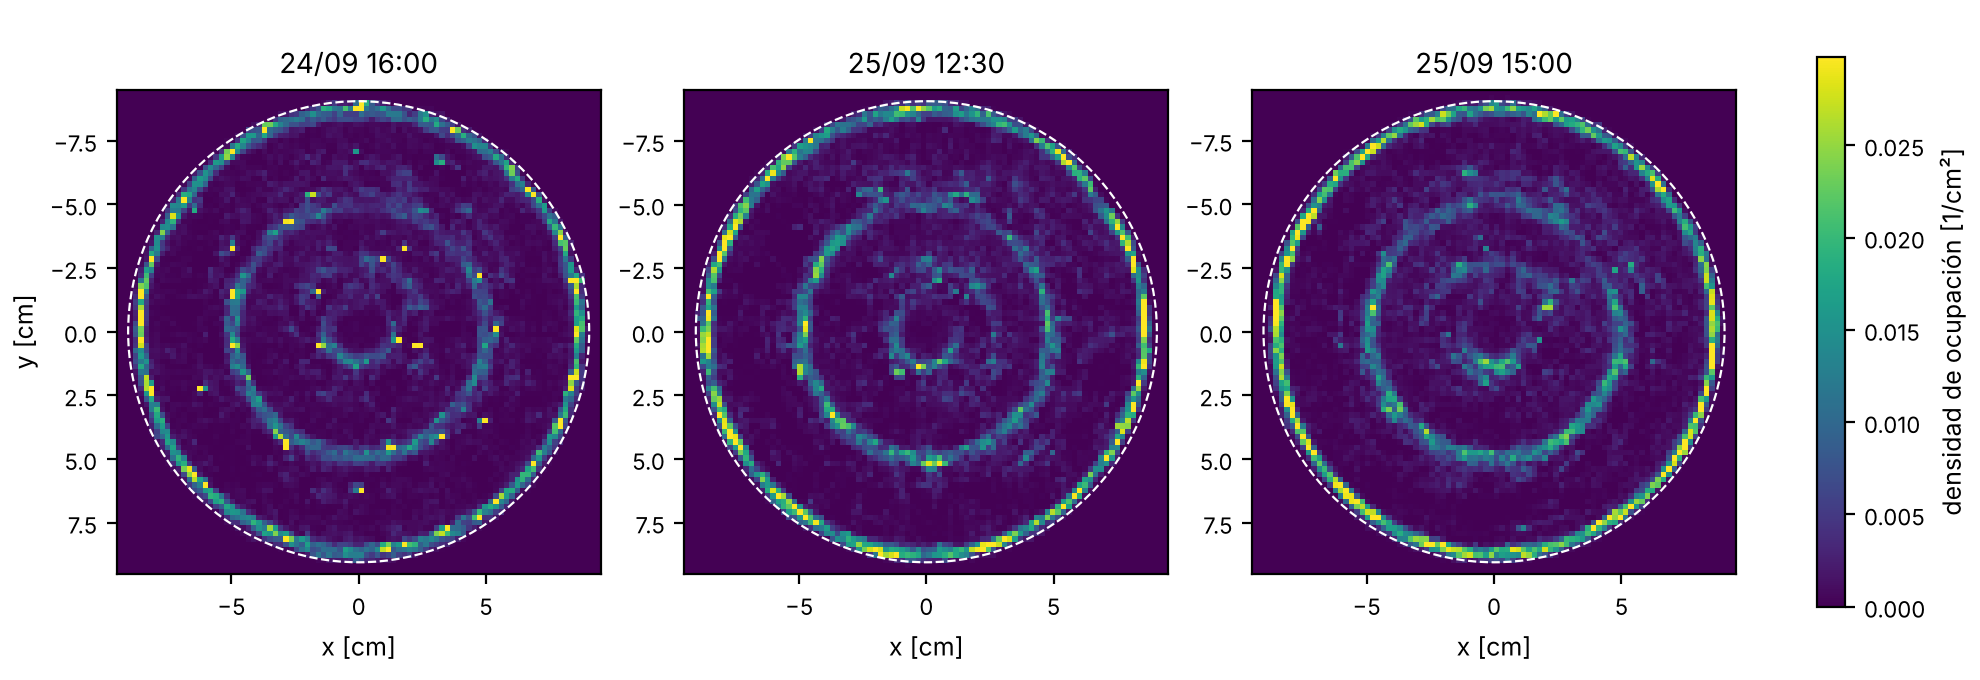
\includegraphics[width=\linewidth]{generado/comparacion/ocupacion.png}
  \caption{Densidad de ocupación de los centros de los robots durante todo cada ensayo. Línea punteada: círculo que pueden alcanzar los centros (radio útil menos el radio del robot).}
  \label{fig:cmp_ocupacion}
\end{figure}
\begin{figure}[H]
  \centering
  \begin{tikzpicture}
    \begin{axis}[width=0.62\linewidth, height=5cm, xmin=0, xmax=1, ymin=0, xlabel={$r/R_{\mathrm{c}}$}, ylabel={densidad relativa}, grid=major, grid style={gray!20}, legend style={font=\footnotesize}, tick label style={font=\footnotesize}, legend pos=north west]
      \addplot [azul, thick, mark=*, mark size=1pt] table [x=r, y=n, col sep=comma] {generado/comparacion/radial_A.csv};
      \addlegendentry{\Cmp{Lab}{A}}
      \addplot [rojo, thick, mark=*, mark size=1pt] table [x=r, y=n, col sep=comma] {generado/comparacion/radial_B.csv};
      \addlegendentry{\Cmp{Lab}{B}}
      \addplot [verde, thick, mark=*, mark size=1pt] table [x=r, y=n, col sep=comma] {generado/comparacion/radial_C.csv};
      \addlegendentry{\Cmp{Lab}{C}}
      \addplot [black, dashed, forget plot] coordinates {(0,1) (1,1)};
    \end{axis}
  \end{tikzpicture}
  \caption{Densidad radial de los centros normalizada por área ($1$ = distribución uniforme); $R_{\mathrm{c}}$ es el radio máximo que alcanzan los centros.}
  \label{fig:cmp_radial}
\end{figure}
